% This is "sig-alternate.tex" V2.0 May 2012
% This file should be compiled with V2.5 of "sig-alternate.cls" May 2012
%
% This example file demonstrates the use of the 'sig-alternate.cls'
% V2.5 LaTeX2e document class file. It is for those submitting
% articles to ACM Conference Proceedings WHO DO NOT WISH TO
% STRICTLY ADHERE TO THE SIGS (PUBS-BOARD-ENDORSED) STYLE.
% The 'sig-alternate.cls' file will produce a similar-looking,
% albeit, 'tighter' paper resulting in, invariably, fewer pages.
%
% ----------------------------------------------------------------------------------------------------------------
% This .tex file (and associated .cls V2.5) produces:
%       1) The Permission Statement
%       2) The Conference (location) Info information
%       3) The Copyright Line with ACM data
%       4) NO page numbers
%
% as against the acm_proc_article-sp.cls file which
% DOES NOT produce 1) thru' 3) above.
%
% Using 'sig-alternate.cls' you have control, however, from within
% the source .tex file, over both the CopyrightYear
% (defaulted to 200X) and the ACM Copyright Data
% (defaulted to X-XXXXX-XX-X/XX/XX).
% e.g.
% \CopyrightYear{2007} will cause 2007 to appear in the copyright line.
% \crdata{0-12345-67-8/90/12} will cause 0-12345-67-8/90/12 to appear in the copyright line.
%
% ---------------------------------------------------------------------------------------------------------------
% This .tex source is an example which *does* use
% the .bib file (from which the .bbl file % is produced).
% REMEMBER HOWEVER: After having produced the .bbl file,
% and prior to final submission, you *NEED* to 'insert'
% your .bbl file into your source .tex file so as to provide
% ONE 'self-contained' source file.
%
% ================= IF YOU HAVE QUESTIONS =======================
% Questions regarding the SIGS styles, SIGS policies and
% procedures, Conferences etc. should be sent to
% Adrienne Griscti (griscti@acm.org)
%
% Technical questions _only_ to
% Gerald Murray (murray@hq.acm.org)
% ===============================================================
%
% For tracking purposes - this is V2.0 - May 2012

%Englisch: Kommentar hier entfernen
\documentclass{sig-alternate}
%Deutsch: Kommentar hier entfernen
%\documentclass{sig-alternate-de}
\usepackage{multirow}

\begin{document}
%
% --- Author Metadata here ---
\conferenceinfo{Advances in Embedded Interactive Systems}{'14 Passau, Germany}
\CopyrightYear{2014} % Allows default copyright year (20XX) to be over-ridden - IF NEED BE.
%\crdata{0-12345-67-8/90/01}  % Allows default copyright data (0-89791-88-6/97/05) to be over-ridden - IF NEED BE.
% --- End of Author Metadata ---

\title{Traffic Flow Optimization via Connected Cars}
%
% You need the command \numberofauthors to handle the 'placement
% and alignment' of the authors beneath the title.
%
% For aesthetic reasons, we recommend 'three authors at a time'
% i.e. three 'name/affiliation blocks' be placed beneath the title.
%
% NOTE: You are NOT restricted in how many 'rows' of
% "name/affiliations" may appear. We just ask that you restrict
% the number of 'columns' to three.
%
% Because of the available 'opening page real-estate'
% we ask you to refrain from putting more than six authors
% (two rows with three columns) beneath the article title.
% More than six makes the first-page appear very cluttered indeed.
%
% Use the \alignauthor commands to handle the names
% and affiliations for an 'aesthetic maximum' of six authors.
% Add names, affiliations, addresses for
% the seventh etc. author(s) as the argument for the
% \additionalauthors command.
% These 'additional authors' will be output/set for you
% without further effort on your part as the last section in
% the body of your article BEFORE References or any Appendices.

\numberofauthors{1} %  in this sample file, there are a *total*
% of EIGHT authors. SIX appear on the 'first-page' (for formatting
% reasons) and the remaining two appear in the \additionalauthors section.
%
\author{
% You can go ahead and credit any number of authors here,
% e.g. one 'row of three' or two rows (consisting of one row of three
% and a second row of one, two or three).
%
% The command \alignauthor (no curly braces needed) should
% precede each author name, affiliation/snail-mail address and
% e-mail address. Additionally, tag each line of
% affiliation/address with \affaddr, and tag the
% e-mail address with \email.
%
% 1st. author
\alignauthor
Thomas Leutheusser\\
       \affaddr{Universität Passau}\\
       \affaddr{Lehrstuhl für Informatik mit Schwerpunkt Eingebettete Systeme}\\
       \affaddr{Innstr. 43}\\
       \affaddr{94032 Passau, Germany}\\
       \email{leutheus@fim.uni-passau.de}
}
% There's nothing stopping you putting the seventh, eighth, etc.
% author on the opening page (as the 'third row') but we ask,
% for aesthetic reasons that you place these 'additional authors'
% in the \additional authors block, viz.

\date{22 November 2014}
% Just remember to make sure that the TOTAL number of authors
% is the number that will appear on the first page PLUS the
% number that will appear in the \additionalauthors section.

\maketitle

\abstract{
	Traffic congestion is an increasingly factor in todays traffic systems. As current traffic information system can only provide a coarse overview over the current traffic situation, the newly emerged technology of Connected Vehicles and its applications to traffic flow optimization is investigated. Vehicular ad-hoc networks and their characteristics are briefly described followed by 6 different traffic optimization techniques, which aim to improve transport statistics such as flow rate, travel times and road safety at different types of granularity.    
}
\keywords{Intelligent Transportation Systems (ITS), Connected Vehicles, V2X, Traffic Flow, Advanced traveler information system (ATIS)}

\section{Introduction}
According to the 2012 Urban Mobility Report of the Texas A\&M Transportation Institute\cite{schrank2012tti} consisting of data from 498 U.S. urban areas, traffic congestion is the major problem for mobility in urban areas with an estimate of 2.9 billion gallons of wasted fuel, 5.5 billion hours more travel time and an assumed cost of \$121 billion. In the EU traffic congestion accounts for an estimate of 80 billion euros a year, according to the European transport policy white paper for 2010\cite{eutraffic}.\\
In order to solve traffic related problems the Federal Highway Administration in the U.S. proposed and defined three general tactics\cite{systematics2005traffic}:
\begin{itemize}
\item Work on current capacity of roads and extend them.
\item Extension of alternative transportation that require less resources (e.g. non-automotive transport).
\item More efficient using of current capacities of cities and roads.
\end{itemize}
Most of the time it is not possible to extend the road network with additional or bigger streets because of the limited available space. Thus the focus is mainly set on the more efficient usage of the current capacities. \\
Intelligent Transportation Systems (ITS) apply information and communication technologies to provide innovative services relating to different modes of transport and traffic management for users to be better informed and make safer, more coordinated and efficient use of the current transport networks.\\ 
Many modern driver assistance systems are already based on an internet connection between cars and a back-end server system. One example for these driver assistance systems is the representation of current traffic information within vehicle navigation systems (e.g. BMW Real Time Traffic Information\footnote{http://www.bmw.de/de/topics/faszination-bmw/connecteddrive/services-apps/rtti.html}) or through the web browser (e.g. Google maps traffic overlay) as seen in Figure \ref{fig:google1}.
\begin{figure} 
\centering
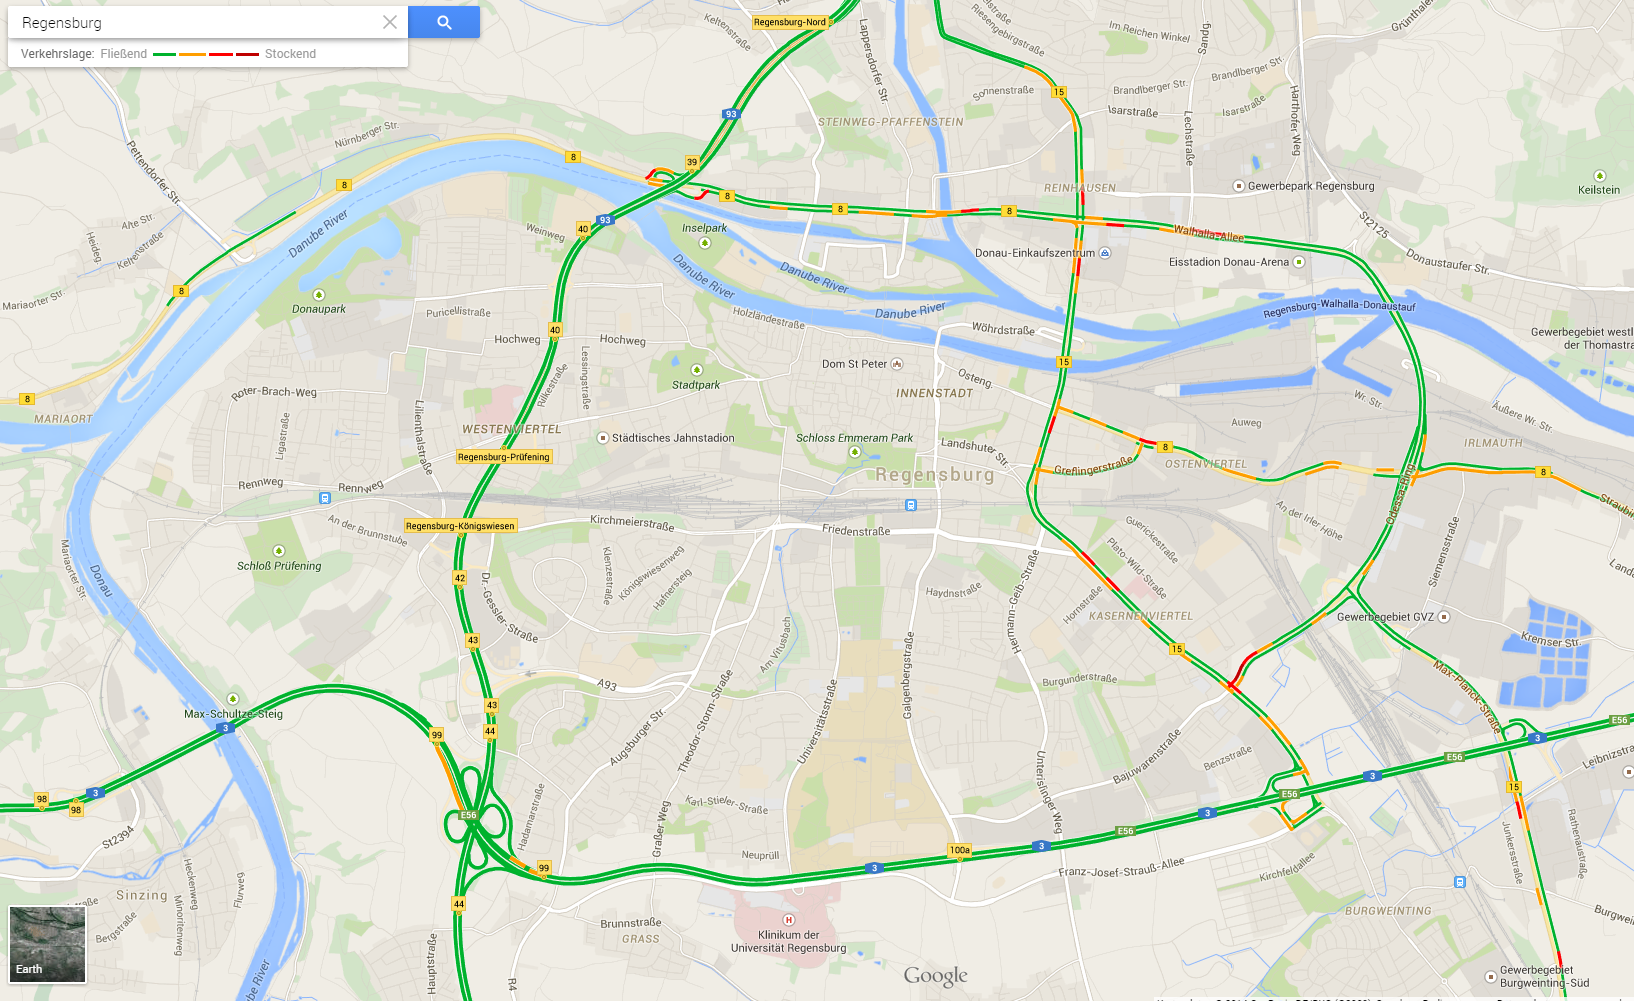
\epsfig{file=google_traffic1.png, width=3.3in}
\caption{Google maps traffic overlay}
\label{fig:google1}
\end{figure}
These mentioned traffic information systems lack the ability to control the traffic on a finer granularity as they can only provide an overview over the current traffic situation. \\
These deficits can be counteracted with Connected Vehicles technology (CV), a relatively new field of study in Intelligent Transportation Systems. Vehicles communicate over different protocols with other vehicles (V2V), infrastructures (V2I) or both (V2X) to form a vehicular ad-hoc network (VANET), where detailed traffic information can be exchanged timely and efficiently. These allow for new types of transport applications ranging from traffic safety systems to infotainment systems. This work focuses on the optimization of traffic flow and congestion relief applications using the mentioned V2X technology, by giving an overview over implementations for different types of techniques.   \\
At first the CV technology and its components are outlined. Then different techniques for traffic flow optimization are explained, followed by a brief discussion of the applications and their usability.  

\section{Connected Vehicles}
Vehicular ad-hoc networks are an application of mobile ad-hoc networks but have their own distinct characteristics which can be summarized as\cite{al2014comprehensive}:
\begin{description}
\item[High mobility] The nodes in VANETs are usually moving at high speeds in "random" directions, but are constrained by the road topology and layout. 
\item[Changing network topology] Due to the high mobility and speeds of vehicles the network topology tends to change frequently. The lifetime of the link between vehicles is affected by the radio communication range and the direction of the vehicles. These rapid changes in link connectivity cause the effective network diameter to be small, while many paths are disconnected before they can be utilized.
\item[Variable network density] The network density in VANET varies depending on the traffic density, which can be very high in the case of a traffic jam or low, as in suburban traffic.
\item[Power constraints] Compared to mobile ad-hoc networks, the power in VANET is not critical because vehicles have the ability to provide continuous power via the long life battery. 
\item[High computational ability] Vehicles can be equipped with a sufficient number of sensors and computational resources such as processors, large memory capacity, advanced antenna technology and GPS. This increases the computational power of the nodes of a VANET which help obtaining reliable wireless communication and accurate information of its position, speed and direction.
\end{description}
To support Intelligent Transportation Systems the IEEE 1609 Family of Standards for Wireless Access in Vehicular Environments (WAVE) have been created. The WAVE standards define an architecture and complementary standardized set of protocols, services and interfaces that collectively enable secure wireless V2X communication. WAVE relies on the IEEE 802.11p standard for the lower physical (PHY) and medium access control (MAC) layers. 802.11p defines a way to exchange data without the need to establish a basic service set as in the 802.11 standards to cope with the high mobility and short link lifetimes between vehicles or infrastructures. Therefore authentication and data confidentiality have to be provided by the upper layers (e.g IEEE 1609). 802.11p uses the 5.9GHz band. \\
Using these communication standards it is then possible to reliably exchange messages between vehicles and infrastructures which is the foundation for intelligent traffic management systems. 
\section{Traffic Flow Optimization }
The main parameters of traffic flow have to be quantified in order to evaluate and compare different aspects of traffic flow. Including others these parameters consist of speed, flow, density, mean speed, and headway. \textbf{Flow} describes the rate at which vehicles pass a fixed point in a time interval. \textbf{Density} is the concentration of vehicles over a fixed length of a roadway. \textbf{Mean speed} is divided into \textbf{time mean speed}, which is the arithmetic mean of vehicle speeds passing a point, and \textbf{space mean speed}, which is the harmonic mean of speeds passing a point during a period of time. The \textbf{headway} is the time that elapses between a vehicle and a following vehicle passing a certain point. \\
Traffic flow can be analyzed at three different levels of granularity. Microscopic traffic flow examines individual vehicles and their properties like speed and position. Macroscopic scale investigates traffic flow characteristics such as density, flow and mean speed on a traffic stream. Mesoscopic models allow the study of large areas with applications such as congestion relief through alternative routes. \\
As a result the types of traffic flow optimization can be applied to different types of granularity. \\
Microscopic optimizations focus on improving the mean travel time for single vehicles by finding optimal vehicle actions such as finding the optimal lane or adjusting the speed to decrease the amount of brakes/accelerations. These optimizations are discussed in chapter \ref{microscopic}\\
The goal of macroscopic optimizations is the increase of throughput and reduced travel times for a given traffic stream. As intersections are the main delay of traffic flows in urban areas the focus is set on uncontrolled and traffic light controlled crossing. These optimizations are discussed in section \ref{macroscopic}.\\
One application to mesoscopic optimizations is the search for optimal routes through congested traffic which is discussed in section \ref{mesoscopic}.

\subsection{Microscopic Traffic Flow Optimizations}
The finest granularity of traffic flow optimizations targets single vehicles and their driving activities. Two different techniques to improve the traffic flow are investigated in this section. Firstly the collaborative interaction to find the optimal driving lane in a highway scenario is described in section \ref{laneselection}. The second technique handles the coordinated approach to a lane drop, which is discussed in section \ref{lanedrop}.
\label{microscopic}
\subsubsection{Optimal Lane Selection}
\label{laneselection}
One driving behavior that can heavily interrupt the flow of traffic are lane changes. The need for lane changes derives from the inequality of desired driving speeds and mandatory lane changes like lane drops or exiting the current road. These lane changes may disrupt the traffic by aggressive maneuvers (i.e. cutting into small gaps) and produce shock wave effects which expand to further upstream vehicles. 
Jin et al.\cite{6856515} propose a cooperative real-time lane selection algorithm named Optimal Lane Selection (OLS) in which connected vehicles share information to improve the system-wide operation of traffic. Well-coordinated lane changes can help maintain desired speeds and minimize shock wave impacts.  \\
This is achieved by calculating the optimal lane target for each vehicle based on its location, speed, lane and desired driving speed. These parameters are transmitted from each car to a roadside communication unit (RSU) which can exchange these real-time information within a certain range. The RSU calculates the optimal lane for each vehicle and sends its optimal lane advice. The drivers then follow the advice by adjusting their lane in order to decrease the overall mount of needed lane changes afterwards. \\
Jin et al.\cite{6856515} tested the algorithm on a simulated 3-way highway of 2000 m length with one roadside communication unit with 300 meters communication range and connected vehicles with a speed of 50 mp/h using the microscopic simulation tool SUMO\cite{sumo}. In the simulation, the mean travel times of different road congestion levels (50\%, 60\%, ... 100\%) with and without their proposed algorithm were compared. Besides the mean travel times, the reduction of energy consumption and the emission of pollutants were simulated (CO, HC, NOx, PM2.5) with MOVES\cite{simulator2010user} (Motor Vehicle Emission Simulator).\\ Their simulation results can be seen in Table \ref{table1}. 
\begin{table}
\centering
\caption{Comparison of results on mean travel times (in seconds) between OLS and non OLS scenarios and different vehicle to capacity ratios}
\begin{tabular}{|l|c|c|c|}
\hline
\multirow{2}{*}{V/C} & \multicolumn{2}{c|}{Scenarios} & \multirow{2}{*}{\% Improvement} \\ \cline{2-3}
                     & NLS Based      & OLS Based     &                                 \\ \hline
0.5                  & 113.0          & 112.4         & 0.57                            \\ \hline
0.6                  & 113.2          & 110.7         & 2.25                            \\ \hline
0.7                  & 114.1          & 109.8         & 3.79                            \\ \hline
0.8                  & 114.3          & 110.5         & 3.35                            \\ \hline
0.95                 & 118.4          & 115.3         & 2.67                            \\ \hline
\end{tabular}
\label{table1}
\end{table}
The simulated mean travel time was reduced by 0,57\% at 50\% road congestion, with up to 3.79\% improvement (118.4 s to 115.3 s) at 70\% of the maximum density. At higher congestion levels the vehicles could not always find the needed space in their suggested lanes, which reduces the success rate of a lane change. At a level of 0.95\% of the maximum capacity of the road, an improvement of 2.67\% in mean travel times was still detected. \\
Similar to the travel times the reduction in pollutants peaked at 70\% road congestion. Energy consumption and CO2 emissions are reduced by around 2.2\% while CO and HC emissions are reduced by up to 17\%. Jin et al. demonstrate how connected vehicles can improve the traffic flow through microscopic actions like well coordinated lane changes. However they do not take into account different penetration rates of interconnected vehicles, which could be useful for the transition years between current and next generation cars. They only simulate their algorithm on a 3-way highway with relatively low speed limit (50 mp/h) and equally treated vehicles. Different simulation runs with trucks, or 2-way highways and  varying penetration rates of V2X technology could have given more insights into the usefulness of this approach. 
\subsubsection{Lane drop merging assistance}
\label{lanedrop}
The second microscopic optimization next to optimal lane changes is the coordinated approach to a lane drop. Schuhmacher et al.\cite{1614269.1614274} provide a Merging assistance algorithm which advices drivers on the individual speed limits and merging positions ahead of a lane drop. The current traffic control strategies in front of lane drop consist of
\begin{description}
\item[Gradual speed limit reduction] Usually used at highway lane drops. The speed limit in front of a lane merge is decreased in several stages to achieve a harmonization of traffic with decreased frictions between vehicles and an increased traffic safety.
\item[Late merge strategy] Drivers are advised to stay in their lane up to the lane drop. This allows the usage of all available lanes until the lane drop. This strategy performs particularly well with heavily congested traffic and low speeds. 
\item [Early merge strategy] Warning signs indicating the lane drop are placed far ahead encouraging the drivers to switch the lane early. This reduces forced merges in the vicinity of the drop. This strategy is preferred at low traffic demands with higher speeds.  
\end{description} 

Schuhmacher et al. present a method which reduces traffic jams and increases the capacity in front of a lane drop by switching to a more effective strategy with the usage of V2X communication for controlled merging procedures.\\ The reference scenario is based on an empiric study\cite{bertini2005empirical} of a freeway lane drop between Heathrow and London, where the passing lane of a 3-way highway transitions to two lanes. The length of the sections and the placement of traffic detectors can be seen in Figure \ref{fig:schuhmacher1} which was taken from \cite {1614269.1614274}. \\
\begin{figure} 
\centering
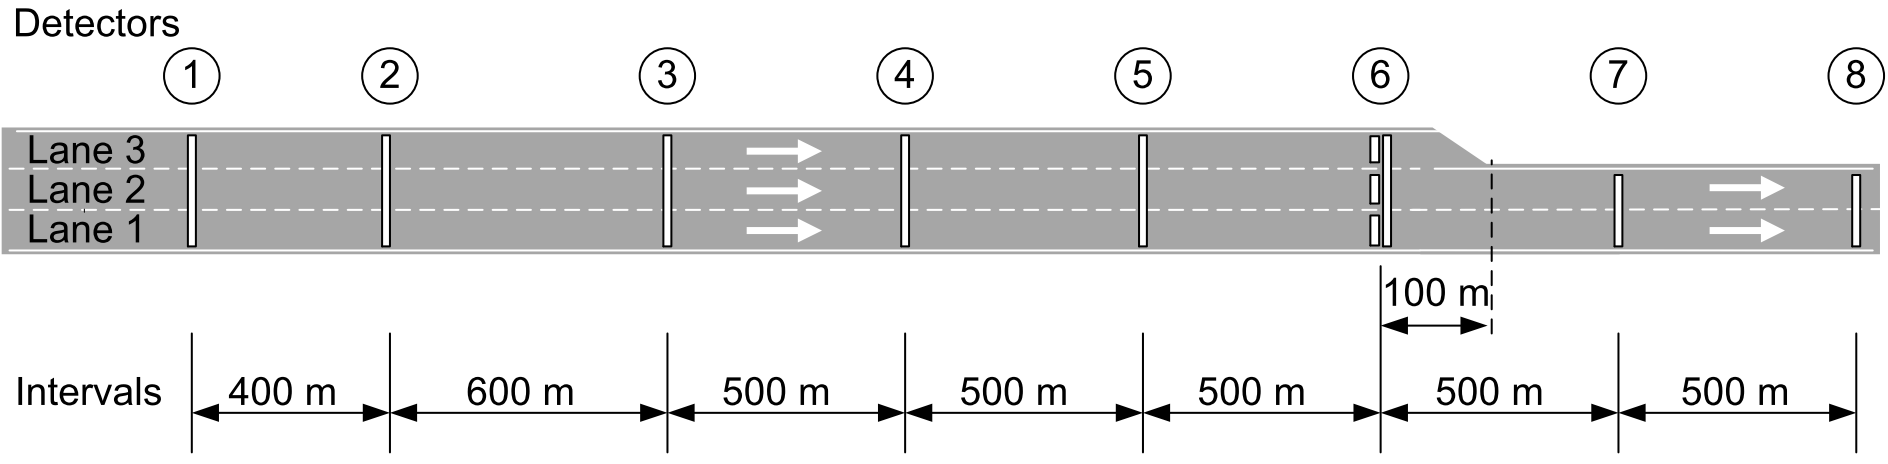
\epsfig{file=schuhmacher_1.png, width=3.3in}
\caption{Reference scenario map with distance intervals}
\label{fig:schuhmacher1}
\end{figure}
Their approach uses a Road-side Unit (RSU) 350 m in front of the lane drop (between detector 5 and 6 of Figure \ref{fig:schuhmacher1}) and On-board units (OBUs) in the vehicles to allow the communication of traffic control messages. The communication parameters are chosen with respect to the IEEE 802.11 family of standards and the 802.11p amendment for Wireless Access in Vehicular Environments (WAVE). Specifically the RSU and OBUs communication range is set to 500 meters. The OBUs are aware of their position (e.g. through GPS) and can not only receive messages from the RSU but also forward messages to other OBUs to achieve a multi-hop communication. \\
The implementation of the merging assistance is a combination of dynamic merge strategies and dynamic gradual speed limits. The main part of the merging assistance algorithm is implemented in the RSU. It analyzes the current traffic conditions by monitoring the time mean speeds of vehicles at the detectors and transmitting traffic control messages  to the OBUs accordingly. These messages consist of the gradual speed limit, the merging positions (e.g. at which point in front of the lane drop the lane switch should occur) and additional messages as "Stay in Lane"  for upstream vehicles and special  "Do Not Pass" messages for heavy vehicles after the merge point, which reduces frictions during the merge procedure as no heavy vehicles are permitted on the lane being merged to. \\
The algorithm works in different stages based on the time mean speed TMS of vehicles at detectors 5 and 6 (the two in front of the lane drop). The TMS are re-evaluated every 5 seconds.
$v_5$ and $v_6$ describe the TMS of detector 5 and 6 respectively. DEM stands for Dynamic Early Merge, DLM for Dynamic Late Merge.
\begin{description}
\item[DEM Stage 1] $v_6 > 80 km/h$ \\
The traffic directly in front of the lane drop (at detector 6) is flowing freely with speeds over 80 km/h. The merge point is set to 400 m in front of the lane drop and a no passing zone for heavy vehicles 400 m ahead of the lane drop is established. 
\item[DEM Stage 2] $v_6<= 80 km/h$ and $v_5>80 km/h$ \\ 
The TMS reduction at detector 6 indicates increasing traffic density resulting in merging problems and braking vehicles. To counteract the merging point is shifted 400m upstream to a distance of 800 m to the lane drop. Ahead of it a "Stay in Lane" zone is established. After it the "Do not pass" rule for heavy vehicles apply. In addition the gradual speed limit reduction is applied to 110, 100, 90 km/h at distances of 2500, 2000, 1000 m ahead of the lane drop, respectively. 
\item[DEM Stage 3] $60 km/h < v_6 <= 80 km/h$ \\ and $v_5 <= 80 km/h$\\
The slightly congested area with decreased TMS between 60 and 80 km/h extended up to detector 5. The distance of the merging point and the "Stay in Lane" zone ahead of it is set to 1300 m. Heavy vehicles are not allowed to pass after the merge point. Gradual speed limit is at 100/90/80 km/h at 2500, 2000, 1000 m.
\item [DLM] $v_6 <= 60 km /h$ \\
Under 60 km/h TMS the traffic condition is assumed to be heavily congested. At this stage it is more efficient to use all lanes as long as possible to maximize the capacity. The merge point is shifted to 100 m ahead of the lane drop, with the "Stay in Lane" and "Do not pass" zones adjusted accordingly. The speed limits are reduced to 90,70,60 km/h at 2500, 2000, 1000 m, respectively.
\end{description}

Schuhmacher et al. simulated their algorithm and the reference scenario with the AIMSUN \footnote{$http://www.aimsun.com/wp/?page\_id=21$} traffic simulator. 
The maximum capacity of a lane was set to 2000 vehicles per hour. The proportion of heavy vehicles was set to 15\% and the maximum allowed speed is 112 km/h (70 mp/h). The traffic demand is increased in three stages every 30 minutes. Firstly 3000 veh/h, which is far under the capacity of 4000 veh/h of the reference scenario. Secondly the demand is increased to 3800 veh/h representing dense traffic close to the maximum capacity. And lastly 4600 veh/h which should result in heavy congestion. \\
In the first simulation run every vehicle is equipped with an OBU and every vehicle obeys the traffic control messages. Compared to a simulation run without the usage of the merging assistance significant traffic improvements were only observed at the highest density of 4600 veh/h. The mean travel time decreased from around 112 sec/km to around 70 sec/km at the end of the simulation run. \\
Figure \ref{fig:schuhmacher2} taken from \cite{1614269.1614274}, illustrates the travel time improvements under different penetration rates of equipped vehicles. 
\begin{figure} 
\centering
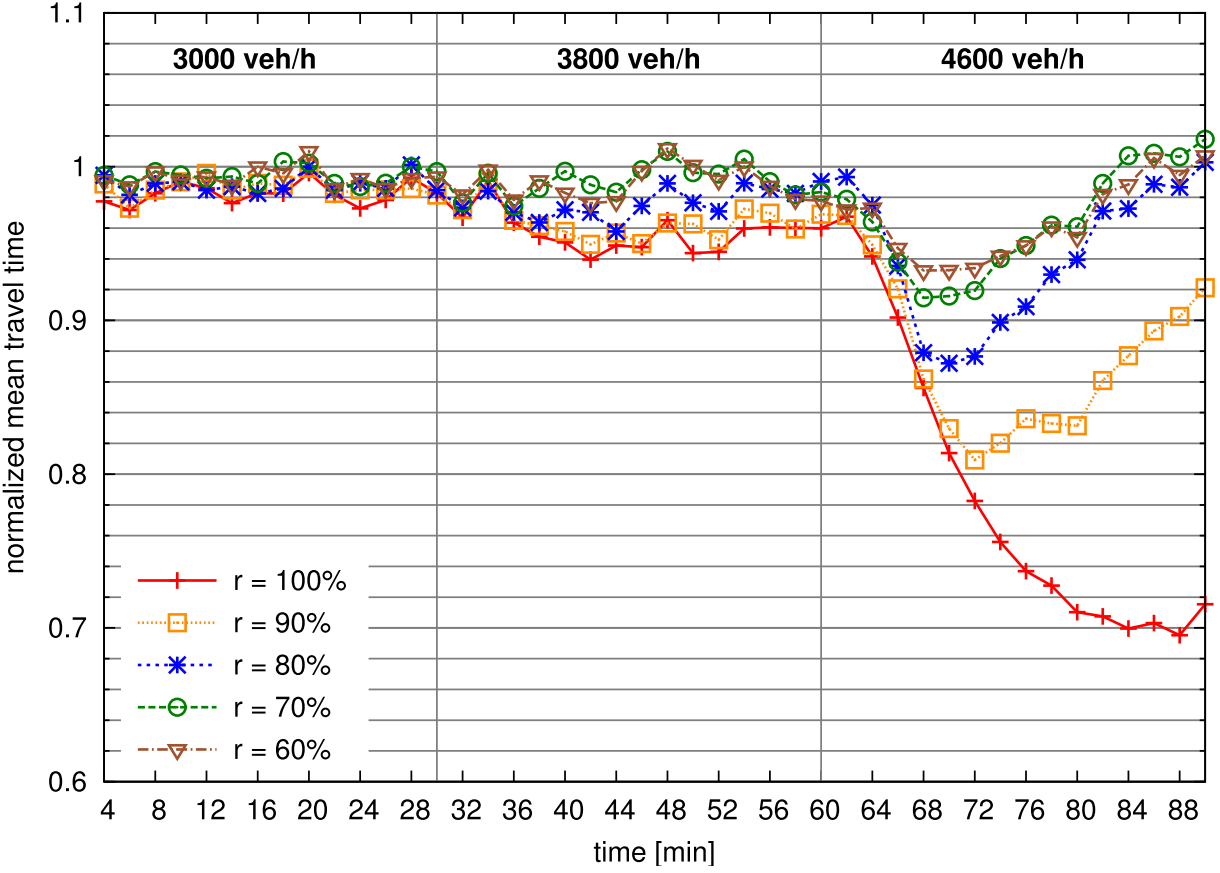
\epsfig{file=schuhmacher_2.png,  width=3.3in}
\caption{Mean flow rates for different penetration rates}
\label{fig:schuhmacher2}
\end{figure}
Next to no improvements where noticeable in low traffic demands (0-30 min.) for each penetration rate. Under higher traffic demands of 3800 veh/h a slight decrease in travel time can be observed. After the beginning of high traffic demand (4600 veh/h, 60-90 min.) the travel time for a ratio of 100\% equipped vehicles decreased by up to 30\%. With a lower ratio of equipped vehicles the mean travel time still decreases by up to 7\% if only 60\% of vehicles are equipped. It can be observed that except for 100\% penetration rate, a traffic breakdown is encountered (e.g. at minute 68 for 80\% penetration rate). The merging assistance application can however help to delay the traffic breakdown and thereby is able to absorb temporary traffic peaks. \\
Schuhmacher et al. present a valid approach to traffic flow optimization by implementing an abstract algorithm for microscopic driver recommendations such as the merging position and adaptive speed limits. Their multi-hop message forwarding communication model can also be extended to eliminate the need of a road side unit. This could be especially helpful for unpredictable lane drops (e.g. accident on lane).


\subsection{Macroscopic Optimization}
\label{macroscopic}
In contrast to the single vehicle, microscopic optimizations of section \ref{microscopic}, this section focuses on traffic improvements on whole traffic streams.
Applications can vary from intelligent traffic lights to intelligent speed limits and speed recommendations at uncontrolled intersections to harmonize the traffic flow. \\
Intersections belong to the most important components of urban road networks with high accident rates and low efficiency in terms of vehicle throughput. Cooperative vehicle infrastructure systems (CVIS) focus on the improvement of safety and flow rates using Vehicle to Infrastructure (V2I) and Vehicle to Vehicle (V2V) communication. This section describes one approach for uncontrolled and one for traffic light controlled intersections. \\

\subsubsection{Cooperative optimization at an uncontrolled intersection}
\label{uncontrolled}
Uncontrolled intersections are the most common types in urban road networks. CVIS are able to get the real-time individual vehicle states and allow the exchange of individual traffic control messages. This can be used to manipulate individual vehicles trajectories to guide them on a non colliding path through the crossing as proposed by Lee et al.\cite{lee2012development}. While this approach can be used for fully autonomous vehicles, it induces problems for self-driven vehicles without accurately driven paths. \\
Cai et al.\cite{6957666} propose a method where drivers are guided by a cooperative negotiated "right of way" information on an installed On-Board Unit (OBU) coupled with speed guidance to preemptively solve conflicts.This reduces the intersections average vehicle delay, number of stops, length of the queue and increases the average speed of vehicles.\\
Vehicles approaching the intersection transmit in small intervals (0.5 s) their current position, speed and desired route to the intersection's traffic controller. For each vehicle the road-side unit calculates an optimal speed, under the assumption that a minimum and maximum speed and a certain acceleration/deceleration rate exists and a minimum headway needs to be retained. These speed guidances are then sent to the OBUs in the vehicles.\\ 
Cai et al. simulated their approach against a non cooperative intersection. Their results are shown in Figure \ref{fig:cai1}. 
\begin{figure*} 
\centering
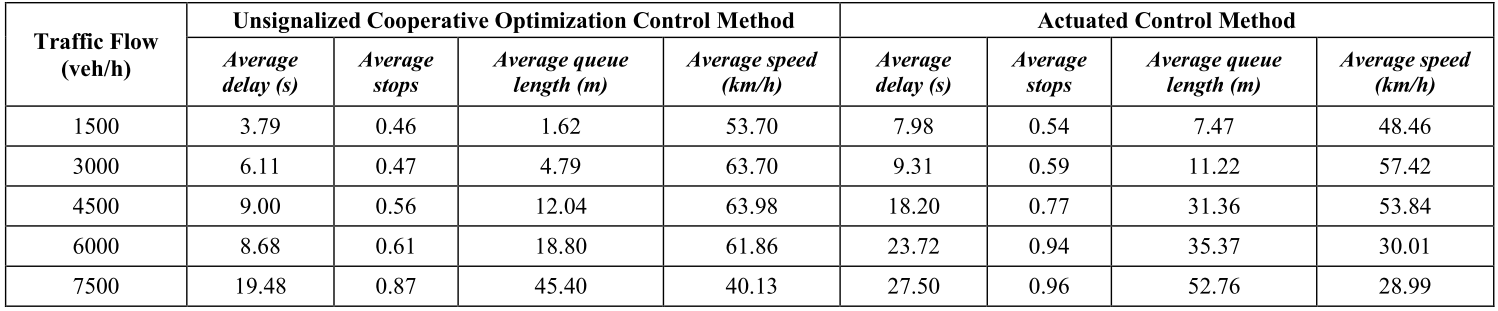
\epsfig{file=cai_1.png, width=6.8in}
\caption{Unsignalized cooperative optimization simulation results}
\label{fig:cai1}
\end{figure*}
The queue length, amount of stops and average delay were decreased while increasing the average speeds of vehicles under all traffic conditions. \\
The results were however achieved under strong assumptions. First of all the interference of pedestrians and bicycles is not considered, which are a strong factor in urban areas. Secondly Cai et al. focus only on isolated intersections without left and right turns or the influence of adjacent intersections. And lastly a penetration rate of connected vehicles of 100\% is assumed. This alleviates the results strongly. \\ 
\subsubsection{Adaptive Traffic Lights}
The message exchange with an infrastructure unit can also be extended to traffic light controlled intersections using the same technique as Cai et al. to convey the state of physical traffic lights directly to a display at the driver. This stands in contrast to computer vision traffic signal detection and recognition, which can be error prone under difficult lighting and weather conditions. Olaverri-Monreal et al.\cite{6263090} present an in-vehicular traffic light implementation with the focus on the design aspects of an Human Machine Interface (HMI). In a driving simulator the design aspects are evaluated regarding the driving performance and acceptance of the novel virtual traffic lights. \\
The virtual traffic lights have to take care of the following characteristics: 
\begin{description}
\item[Design] The design components size, shape, color, composition, lighting and contrast have to provide a clear and easy to understand message. A Head Up Display (HUD) was chosen to display the few required elements (distance to traffic light, traffic light state). 
\item[Placement and operation] To avoid a road vision obstruction in the central field of view, the images were projected 2.5 to 4 meter away from the drivers eyes in the lateral field of view.
\item[Maintenance and uniformity] The maintenance of the system is similar to other electronic devices in the vehicle. The installation of the sensors and the V2V communications allows similar functioning of all the traffic lights virtually displayed. 
\item[Color code] Luminance requirements need to be followed to ensure that the projected images are visible in all weather conditions. 
\item[Signal timing] Vehicles are detected at traffic lights, which is used to determine priority and traffic light phase duration. The virtual traffic light system uses a robust detection system based on beaconing and location tables through a geographic routing protocol. Additionally traffic light warnings alert the driver if a traffic violation occurs. Each vehicle maintains an internal database with information about intersections where a virtual traffic light can be created. If a vehicle approaches a intersections and does not detect a virtual traffic light, they consult their location table and the road map topology to infer crossing conflicts and then create a collaborative virtual traffic light. This requires lane-level accuracy on the location tables and digital road maps with lane-level information topology. 
\end{description}
Two in vehicular traffic light designs can be seen in Figure \ref{fig:trafficlight1}. Design A1 and B1 show a traffic light ahead warning with a label indicating the remaining distance. Design A2 and B2 show the driving priority through green or red colored arrows. Design B3 shows the driving permissions through a traffic light image. 
\begin{figure} 
\centering
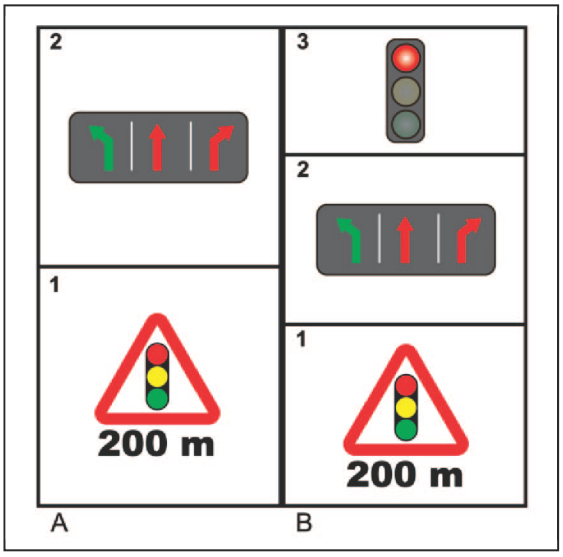
\epsfig{file=traffic_light1.png, width=3.3in}
\caption{Different virtual traffic light designs}
\label{fig:trafficlight1}
\end{figure}
This design was then tested in an urban driving simulator. An in vehicle-view of an virtual traffic light is shown in Figure \ref{fig:trafficlight2}.
\begin{figure} 
\centering
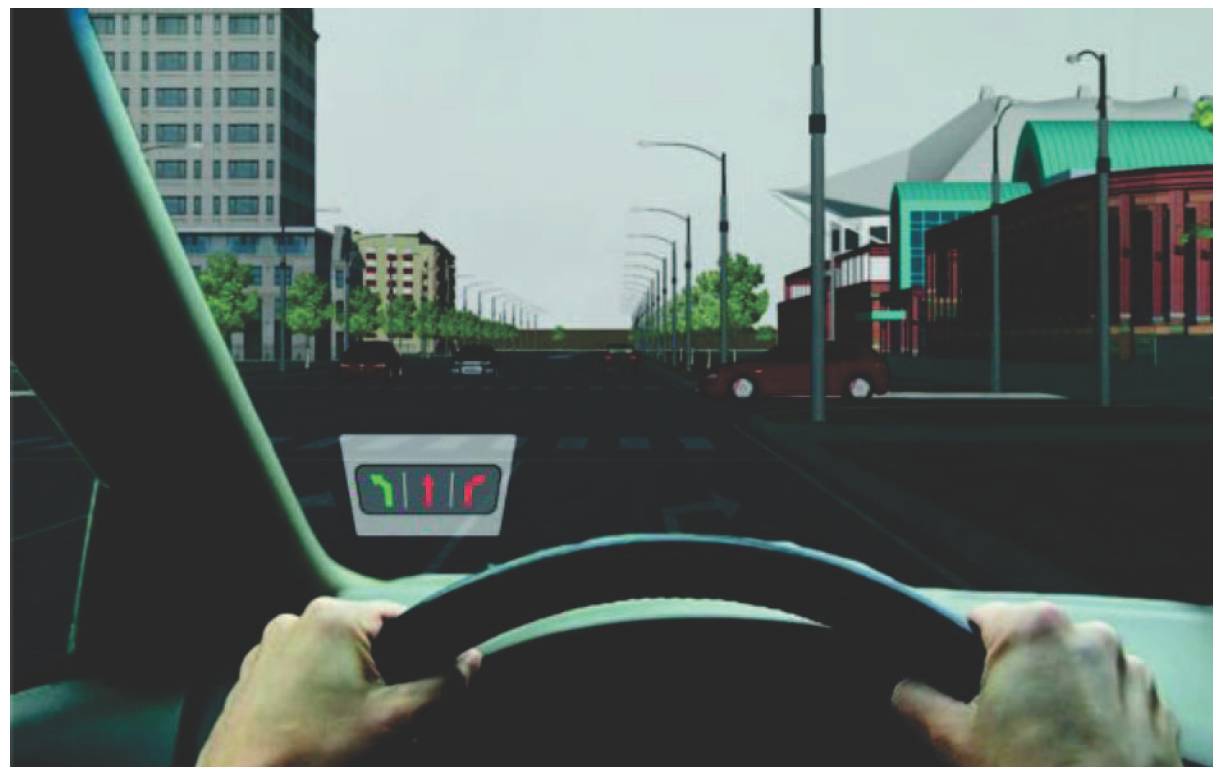
\epsfig{file=traffic_light2PNG.png, width=3.3in}
\caption{In-vehicle view of the virtual traffic light projected on the windshield}
\label{fig:trafficlight2}
\end{figure}
To determine the driving performances Olaverri-Monreal et al. focused on speed metrics and brake activity, because the ability to adapt to new road circumstances such as traffic signs or intersections can be observed in the variation of speed. \\ From the 10 tested persons 9 declared the presented information as clear and intuitive and was not considered distracting or unsafe. The brake activity and deceleration rate differed only slightly from the simulation run with the physical traffic lights. In general the test group adapted well to the shift from physical to virtual traffic lights\\

\subsubsection{Adaptive traffic light control for priority vehicles}
\label{trafficlights}
Intelligent traffic lights can further be extended to not only improve the traffic flow at intersections based on demand, but to also control the traffic flow based on different parameters such as the presence of emergency vehicles approaching this intersection. Top priority is given to emergency vehicles and their demanded lanes. This enables priority vehicles to drastically reduce their travel time to destination especially in heavily congested areas.\\ 
Ahmed et al.\cite{6799827} compare two different scheduling schemes for intelligent traffic lights which receive the following information from the vehicles. 
\begin{itemize}
\item Total number of vehicles within a lane.
\item Vehicle type (i.e. priority or non priority)
\item Total travel time of a vehicle
\item Initial assigned deadline of each vehicle
\end{itemize} 
The first scheme is a static Fixed Priority (FP) algorithm, where vehicles types are assigned to different priority levels. 
\begin{itemize}
\item High Priority Vehicles (HV)
\item Medium or Moderate Priority Vehicles (MV)
\item Low Priority Vehicles (LV)
\item Nil Priority Vehicles (NV)
\end{itemize}
The static algorithm firstly serves all edges with HV vehicles present, followed by MV, LV and lastly NV type vehicles. \\
The second algorithm proposed by Ahmed et al. also classifies vehicles into priority classes, but uses the deadlines of processes to prioritize vehicles. HV vehicles are assigned lower deadlines than MV vehicles. LV type vehicles get intermediate deadlines and NV type vehicles obtain the highest deadline. The algorithm then serves the intersection edge which has the vehicle with the lowest deadline first. This Earliest Deadline First (EDF) approach is a dynamic implementation as it makes its decision based on the dynamic deadlines of priority vehicles.\\
Ahmed et al. simulated the two scheduling schemes and the standard static traffic lights using the simulator SUMO\cite{sumo}. They used a complex network as shown in Figure \ref{fig:ahmed1} taken from \cite{6799827}. 
\begin{figure} 
\centering
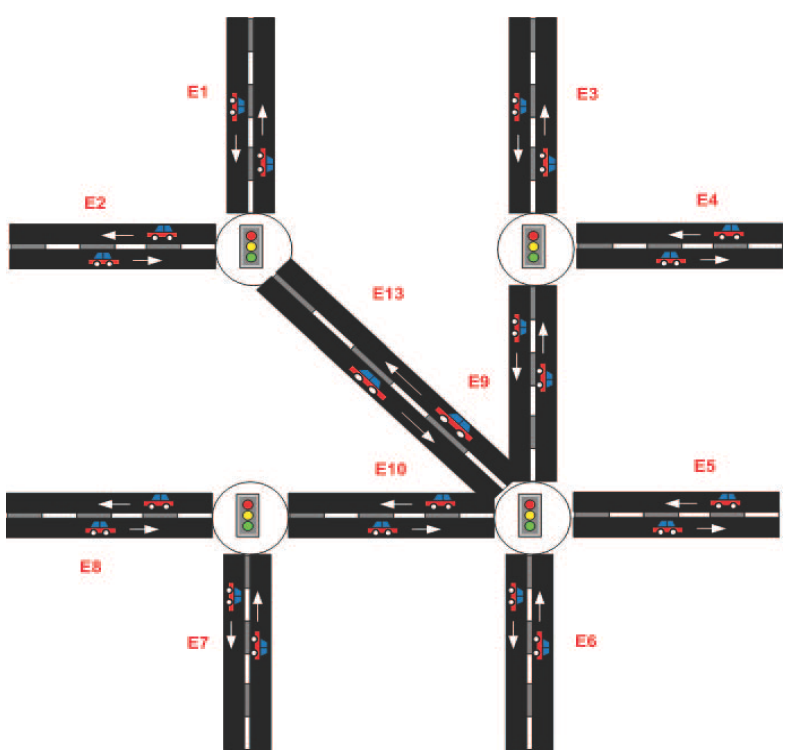
\epsfig{file=ahmed1.png, width=3.3in}
\caption{Network containing complex intersections}
\label{fig:ahmed1}
\end{figure}
Different traffic intensities were simulated and the percentage of priority vehicles was set to 14\% of the total traffic. In their results seen in Figure \ref{fig:ahmed2} it can be seen that both the adaptive traffic light implementation outperform the typical traffic lights in terms of mean waiting steps, mean trip time and mean speed for priority vehicles. It has to be noted that the gain for priority vehicles is achieved at the cost of no and low priority vehicles. 
\begin{figure*} 
\centering
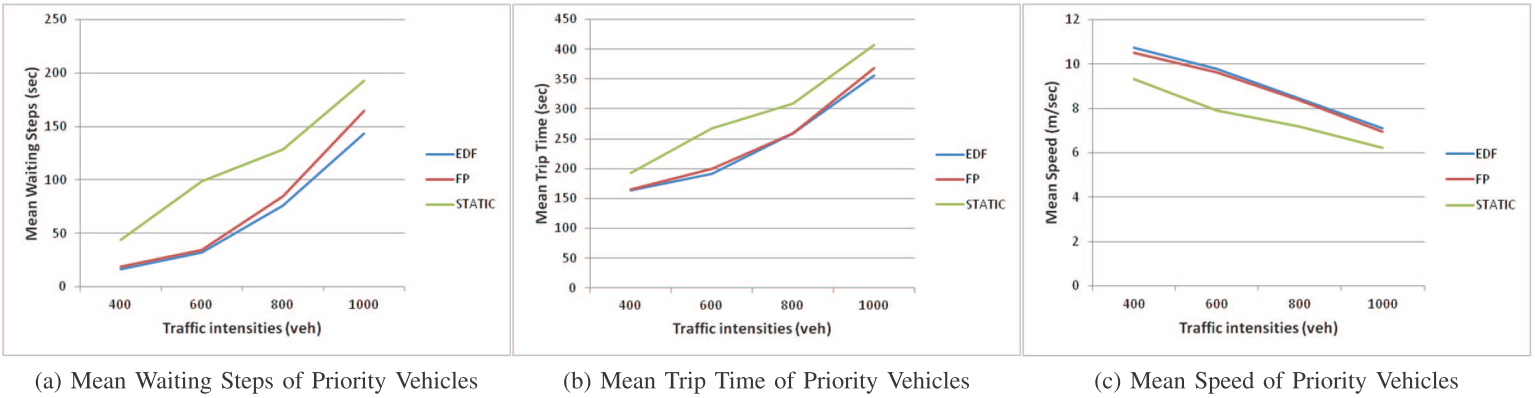
\epsfig{file=ahmed2.png, width=6.8in}
\caption{Simulation results for a network of complex intersections using FP, EDF and static scheduler}
\label{fig:ahmed2}
\end{figure*}
The amount of mean waiting steps (Figure \ref{fig:ahmed2}a)) are reduced by up to 50\% compared to the static traffic lights. The mean trip time and mean speed parameters of priority vehicles are also greatly improved using EDF and FP schedulers. Also the EDF scheduler performs slightly better than the Fixed Priority implementation.\\ 


\subsection{Mesoscopic Optimization}
\label{mesoscopic}
The previously mentioned optimizations had in common that the vehicles were directly in the communication range of a single infrastructure unit (e.g. one RSU at \ref{laneselection}, the intersection control at \ref{uncontrolled} or the intelligent traffic lights at \ref{trafficlights}). For mesoscopic models, where the investigated area exceeds this communication range, a reliable and efficient method is required to exchange traffic information timely with as much vehicles as possible. As it is assumed that all V2X enabled vehicles have the ability to share their positional data (e.g. through GPS) current communication models favor Geocast over Cluster-Based or Broadcasting models. Kaiwartya et al.\cite{6776965} provide an overview and classify the current Geocast routing protocols. \\  
With reliable and timely traffic information over large areas it is possible to identify and avoid congested roadways. Finding the fastest vehicular route to a destination has several benefits, such as reducing traffic congestion, fuel consumption and traffic emissions.\\
Noori et al.\cite{6799873} investigated a large scale V2X enabled urban area and developed an dynamic route planning algorithm using V2X communication and real-time traffic information. \\
To achieve this task their proposed methods consists of the following requirements:
\begin{itemize}
\item Every road segment has a Road-side-unit at the start and at the end of the segment. 
\item Every road segment has a Ideal Traveling Time (ITT). The ITT is the time required for a car to go from the beginning of the street to the end of the street under ideal circumstances (when the road is empty and with the maximum allowed speed). This can be calculated via the length of the road segment and the allowed maximum speed. 
\item Every road segment has a Current Traveling Time (CTT). The CTT is calculated by building the average over the traveling time for the 5 last recent cars in the street. When a vehicle enters a road segment, the RSU transmits the current time and date to the vehicle. The car holds this message and periodically broadcasts this message until it arrives at the end of the segment. The RSU at the end point calculates the traveling time by subtracting the real time and the starting time for this car. 
\item The CTT for every road segment is broadcasted and made available to all vehicles in the urban area. 
\item If a RSU did not receive any data or the time of the last transmission is greater than the ITT, the RSU assumes that there is no car in the street and assigns a CTT equal to the ITT of the segment.
\end{itemize}

With these requirements the road network forms a weighted graph, with the current traveling time labeling the weight for the edges. The search for the fastest route is then a classic shortest path problem. Noori et al. have chosen the A* algorithm to find the shortest path with the CTT as their cost function. To allow a dynamic route planning this shortest path is re-evaluated after every simulation step with the newest broadcasted CTTs. These changes to the car's route happen until the car arrives at the destination. \\
Noori et al. imported a realistic vehicle traffic and traffic related information model of the city of Cologne from the TAPAS-Cologne project from the German Aerospace Center, Institute of Transportation System and OpenStreeMap data covering  approximately an area of 400 $km^2$ into the traffic simulator SUMO. This dataset contains car traffic from 24 hours consisting of 700.000 individual vehicle trips. \\
Their simulation scenario investigates the impact of the route planning algorithm at the peak traffic demand between 6 a.m. till 8 a.m. The city map is divided into several zones based on the traffic status. After that 20 different zones are selected and one vehicle is added to each zone with a traveling distance of 5 km. \\
Three simulations are done to observe the vehicles traveling time:
\begin{itemize}
\item In the first run, only the mentioned 20 vehicles travel the city of Cologne without any traffic lights or other vehicles to measure the ideal traveling time.
\item The real traffic of cologne is simulated with over 250.000 individual vehicles with the 20 vehicles included, in order to simulate the vehicles travel time without the route planning algorithm.
\item Lastly the dynamic route planning is enabled for the 20 vehicles and their travel time is observed. 
\end{itemize}
Figure \ref{fig:noori1} illustrates the simulated travel times for the 20 selected vehicles. 
\begin{figure} 
\centering
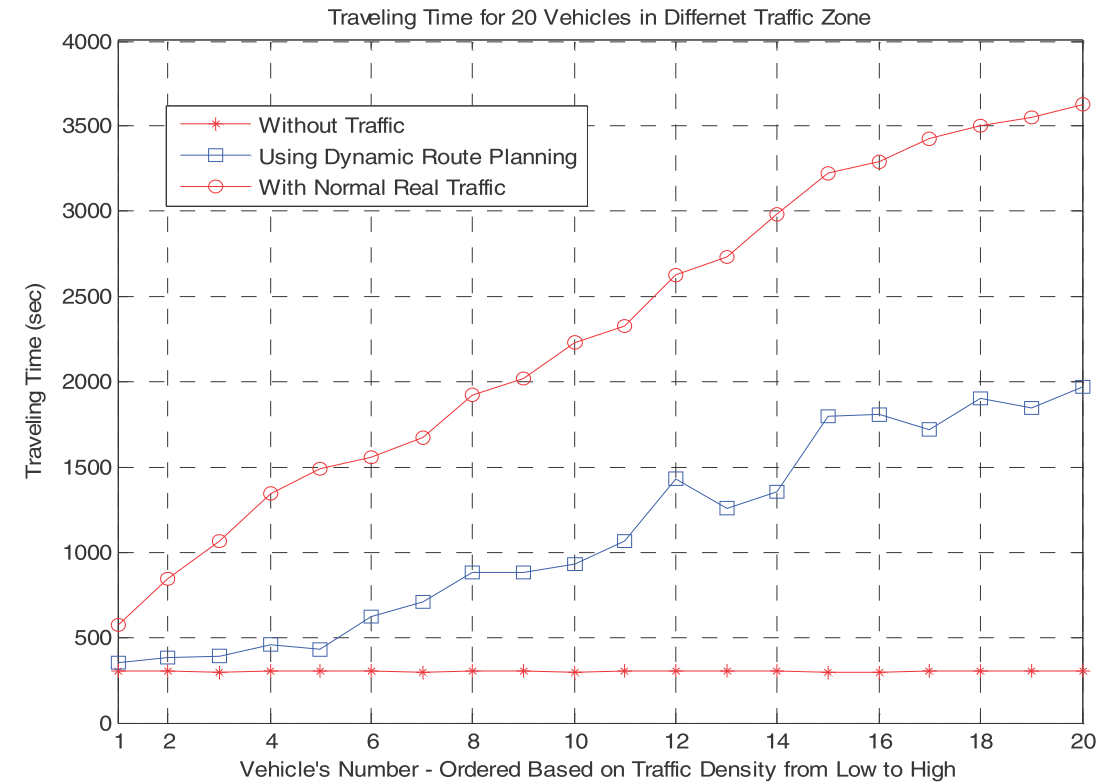
\epsfig{file=noori1.png, width=3.3in}
\caption{Travel time of vehicles based in different traffic densities}
\label{fig:noori1}
\end{figure}
A reduction of 41.12\%  in average travel time in low traffic areas (car number 1 - 7), 52,84\% for medium traffic (car number 7 - 14) and 60,79\% for high traffic areas (car number 14-20) compared to the real traffic of cologne was achieved in the simulation run. These results show that under perfect circumstances (traffic information is instantaneously broadcasted, all vehicles receive traffic information, every road segment is V2X equipped) the travel time in dense urban areas can be drastically reduced for a few selected cars. The impacts when large fleets of dynamically routed cars use this system are not discussed. \\ The obtained results are likewise only achievable in simulation runs, because the assumption that every single road segment is equipped with a RSU at the start and end can realistically not be achieved in the near future. 


\section{Discussion}
The research in ITS is still in its early stages. Foundations for large scale VANETs such as routing protocols and security concerns need to be ensured before the focus can be shifted to more complex traffic safety and traffic management systems. Secondly applications to traffic flow optimizations can currently only be simulated, which gives a certain blur to the expressiveness of the results. Still the provided techniques forecast the immense opportunities that Connected Vehicles can give to traffic safety and traffic efficiency. \\
Some topics that were not addressed in the discussed applications but need to be evaluated is firstly the presence of traffic participants such as bicycles and pedestrians. Especially the approach to in-vehicular traffic lights does not conform well with non-motorized and unconnected road members. An exemplary solution, with the increasing possession of smart phones, could be to involve mobile data into the creation of traffic light control messages. \\
Lastly it needs to be considered how well traffic control advices are accepted and carried out. For example the question arises how well the optimal lane change algorithm performs with single individuals ignoring or even acting oppositely to the advices.   

\section{Conclusion}
This work provides an overview over some example applications to traffic flow optimization using connected vehicles. These applications were divided into different classes based on the type of optimization. For each granularity one or more systems were examined and their results were presented. 


%%%%%%%%%%%%%%%%%%%%



%
% The following two commands are all you need in the
% initial runs of your .tex file to
% produce the bibliography for the citations in your paper.
% ENGLISCH: Kommentar dieser Zeile entfernen
\bibliographystyle{abbrv}
% DEUTSCH: Kommentar dieser Zeile entfernen
%\bibliographystyle{abbrv-de}
\bibliography{bibliography}  % bibliography.bib is the name of the Bibliography in this case
% You must have a proper ".bib" file
%  and remember to run:
% latex bibtex latex latex
% to resolve all references
%
% ACM needs 'a single self-contained file'!
%
%APPENDICES are optional
%\balancecolumns

% This next section command marks the start of

%\balancecolumns % GM June 2007
% That's all folks!
\end{document}
